
\chapter{Introduction}

The complexity of hardware and software is increasing as the years are passing. With increase in complexity, likelihood of errors is much greater. A major goal of software engineering is to enable developers to implement systems which operate reliably despite the complexity. One of the ways to achieve this is by using \emph{formal methods} \cite{clarke1996formal}. Formal methods are mathematically based techniques, tools and languages for describing and verifying the system. These techniques can greatly increase our understanding of a system by revealing incompleteness, ambiguities and inconsistencies that may go undetected otherwise \cite{hall1990seven}.

Single core processor's speed is limited by the physics of semiconductors. High performance computers are being designed using multiple cores to reach the high computation goals. In multicore systems, applications are designed to execute in parallel, and computation speed is achieved by parallel computation. The parallel computation increases complexity of software and hardware. Research industry is working on developing tools and techniques to reduce complexity and detect possible error cases. In this work we have analysed an embedded multicore Digital Signal Processor (DSP) architecture and software, and developed \emph{model checking} techniques. DSPs are processors with special functional blocks to handle digital signals. A digital signal is a sequence of discrete values which represent a physical signal, for example, representing a radio signal or audio signal. Digital signal processing can be enhanced by features like fixed point arithmetic, coprocessors and dedicated registers. Standard C language does not have explicit support to handle these features. Industry and researchers have defined extensions like Embedded-C and DSP-C to add these features to standard C. We have added support for DSP-C in our bounded model checking tool to process DSP-C based programs. We will present multicore, parallel processing, DSP functionality and DSP-C in later chapters.

\emph{Model checking} is a formal method for verifying logical correctness. Proving logical correctness can be very effective in development process since testing lacks the coverage \cite{zhu1997software}, peer review is error prone and costly. For example as we can see in \autoref{fig:example:test:coverage:code}, the function $greatest\_common\_divisor$ can iterate in while loop based on values of x and y, which are dynamic values. There are $2^N * 2^N$ possible inputs and $2^N$ outputs, where N is number of bits in int data type. In large software it is impractical to cover all the inputs, outputs and behaviours of each function and module. There are alternative approaches in testing, like code coverage techniques and white-box testing, which can provide some assurance of behaviour but testing cannot prove the correctness.


\begin{figure}[h]
    \centering
    \tikzstyle{module}=[draw, text centered, minimum width=3em, minimum height=1.6em, rectangle, rounded corners]
    \tikzstyle{decision} = [diamond, draw, text width=4.5em, text badly centered, node distance=3cm, inner sep=0pt]
    \tikzstyle{line}=[draw, -latex]
    \begin{tikzpicture}[node distance=1.5cm, auto]
    \node (begin) [module] {
       \begin{lstlisting}
int greatest_common_divisor(int x, int y)
{
      while(x > 0 && y > 0)
      {
          if(x > y)
              x=x-y;
          else
              y=y-x;
      }

      return (x+y);
}
       \end{lstlisting}
    }; 

    \end{tikzpicture}
   \caption{Function to find greatest common divisor}
   \label{fig:example:test:coverage:code}
\end{figure}

Verification techniques are being employed extensively in hardware and embedded system development. Since, hardware and embedded systems are designed, developed once and mass produced, and bugs in implementation cannot be fixed once produced. Even a single bug in system may lead to recall of all the products. Also, embedded systems have become part of our regular life. For example, microwave oven at home to safety critical systems like power plant controller or flight controllers in aircraft. A single bug in these systems can lead to fatal disasters. Verification techniques can help us to identify possible error cases. In embedded systems, verification can identify problems like checking if array access is within the defined array bound, dangling pointers, arithmetic overflow or underflow and if it is a multicore systems, data races, deadlocks and many other properties can be verified \cite{werner2010correctness, post2007integrated, vasudevan2008static}.


\begin{comment}
\begin{figure}[h]
    \centering
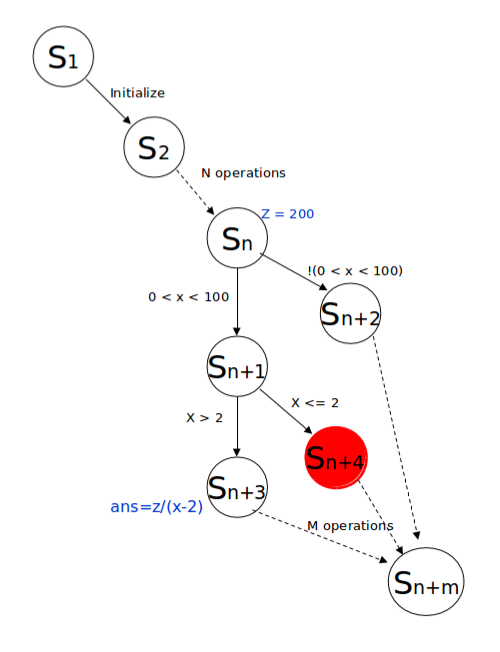
\includegraphics[scale=0.5]{images/statemachine.pdf}
   \caption{State machine example}
   \label{fig:state:machine}
\end{figure} 

For example consider state-machine in \autoref{fig:state:machine}, expressions in blue represent the operations performed in the state and guards, in black, on edges represent the conditions for moving on to next state. Model checking tool can preprocess these expressions and guards, and suggest if any of the error states are reachable. In the example state machine, states coloured in red are error states. Reaching state $S_{n4}$, which is coloured red, will cause an error in the system. Model checker can verify if the $S_{n4}$ is reachable and if system can enter an error state.
\end{comment}

\begin{figure}[h]
    \centering
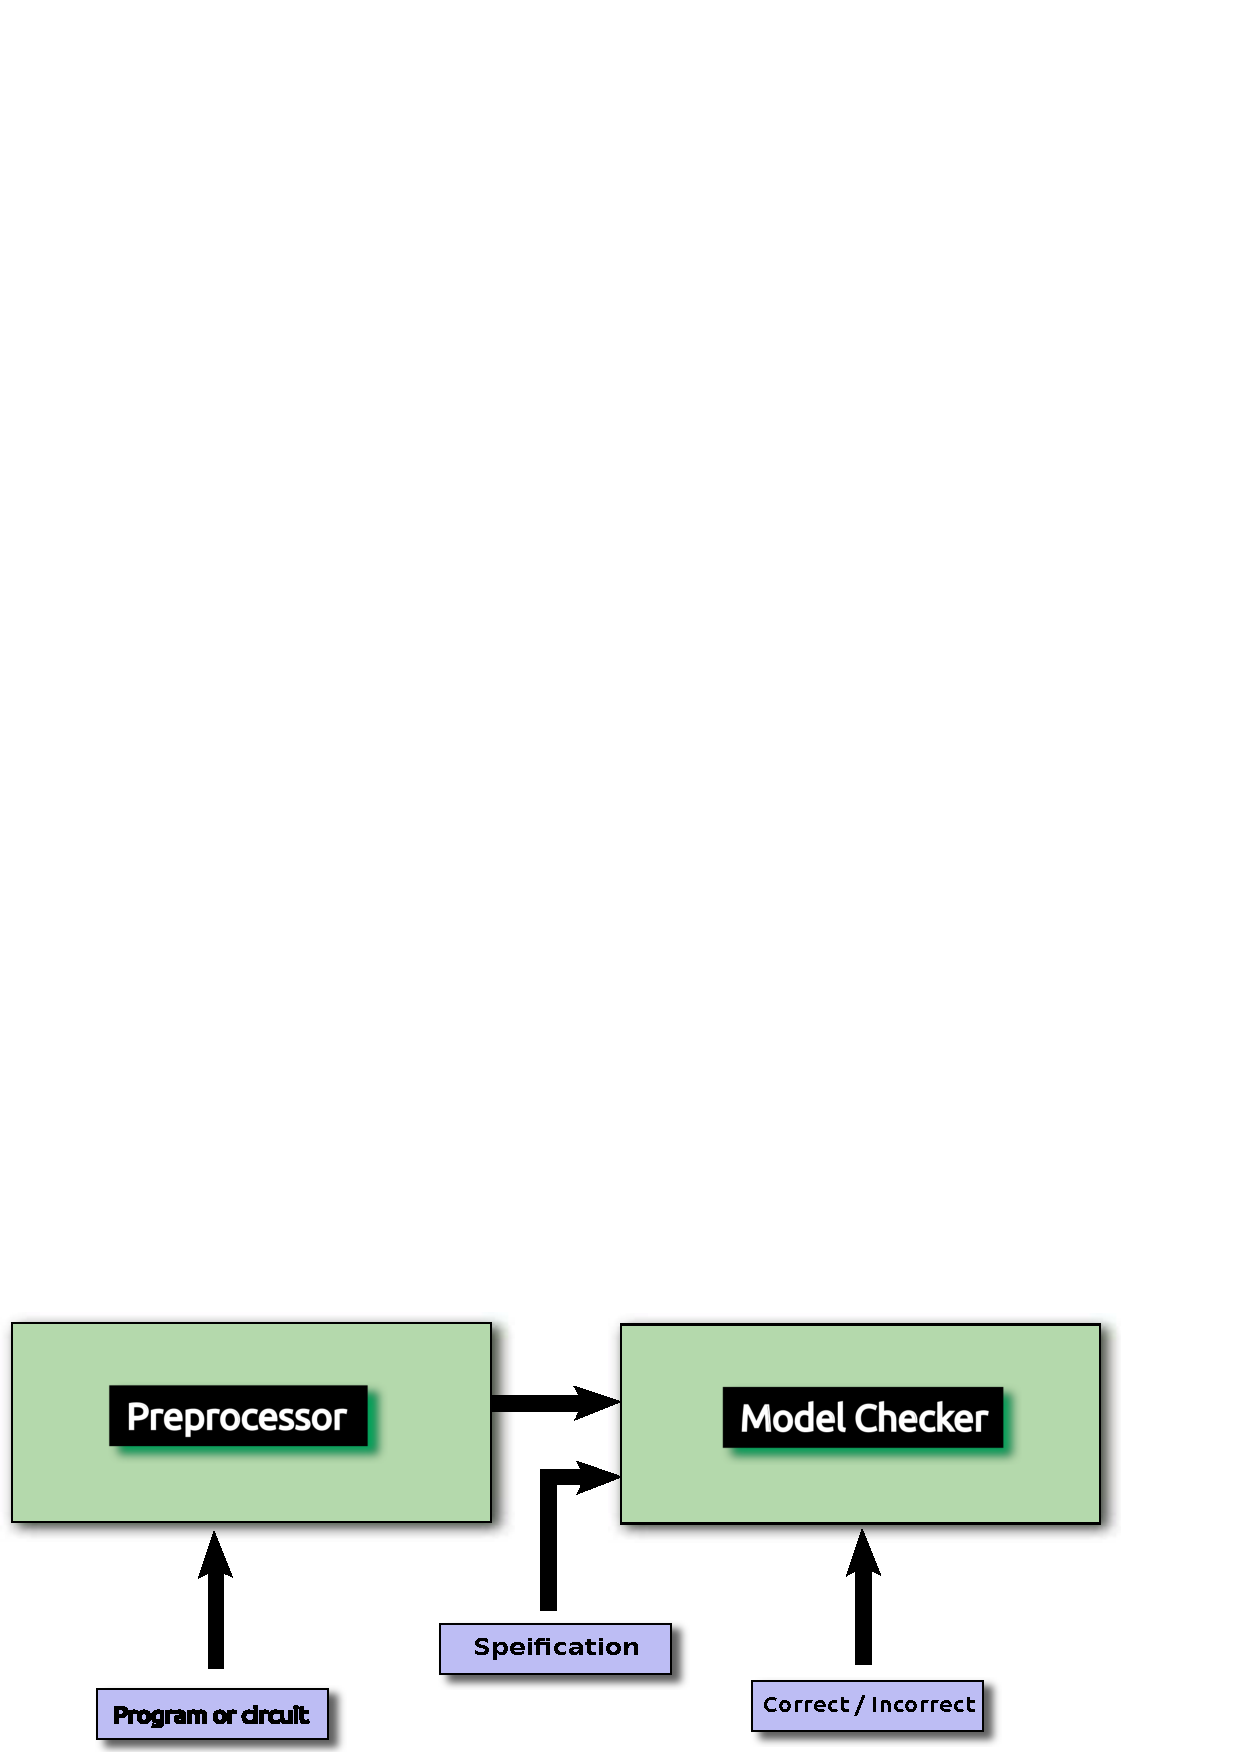
\includegraphics[width=\linewidth]{images/modelChecking.pdf}
   \caption{Model checking \cite{clarke2008birth}}
   \label{fig:model:checking}
\end{figure}

Model checking \emph{statically analyses} the implementation and asserts on properties of the logic. \autoref{fig:model:checking} shows the block diagram of model checking. A model checker reads program or circuit logic, converts it into a formula and compares it with the specification. Model checker matches logic and specification, and tells the implementation is incorrect if the logic differs from specification. Model checking is used to detect undesired behaviours of the system.

Software model checking is complex since it operates based on information available statically, without running programs and programs contain code segments controlled by dynamic conditions \cite{godefroid2005software}. Software model checking also has to cope up with loops which are bounded with run-time conditions, for instance, while loop in function $greatest\_common\_divisor$ (\autoref{fig:example:test:coverage:code}) is bounded by values of x and y. Dynamically bounded programs can be verified using \emph{Bounded Model Checking (BMC)}, which considers a static bound on loops \cite{biere2003bounded}. For instance \autoref{fig:example:test:coverage:code:loopunrolled} shows $greatest\_common\_divisor$ with loop unrolled. In this example static bound used for loop unrolling is 5. As we can see assert statement at the end is used to verify if bounding limit is not enough. We should note that bounded model checking does not guarantee complete program correctness, since it verifies programs within a bounds.


\begin{figure}[h]
    \centering
    \tikzstyle{module}=[draw, text centered, minimum width=3em, minimum height=1.6em, rectangle, rounded corners]
    \tikzstyle{decision} = [diamond, draw, text width=4.5em, text badly centered, node distance=3cm, inner sep=0pt]
    \tikzstyle{line}=[draw, -latex]
    \begin{tikzpicture}[node distance=1.5cm, auto]
    \node (begin) [module] {
       \begin{lstlisting}
int greatest_common_divisor(int x, int y)
{
     if(x > 0 && y > 0)
     {
          if(x > y)
              x=x-y;
          else
              y=y-x;

          if(x > 0 && y > 0)
          {
              if(x > y)
                  x=x-y;
              else
                  y=y-x;
   
              if(x > 0 && y > 0)
              {
                  if(x > y)
                      x=x-y;
                  else
                      y=y-x;

                  if(x > 0 && y > 0)
                  {
                      if(x > y)
                          x=x-y;
                      else
                          y=y-x;

                      if(x > 0 && y > 0)
                      {
                          if(x > y)
                              x=x-y;
                          else
                              y=y-x;

                          assert(x > 0 && y > 0);
                      }
                  }
              }
          }
     }

     return (x+y);
}
       \end{lstlisting}
    };

    \end{tikzpicture}
   \caption{Loop unrolled greatest common divisor function}
   \label{fig:example:test:coverage:code:loopunrolled}
\end{figure}



\emph{CBMC} is a Bounded Model Checking tool which can process C and C++ programs and verify different properties \cite{website:cprover:cbmc, clarke2006ansi, Clarke04atool}. It converts programs into intermediate forms which are called \emph{goto-programs}\index{goto-program}. The goto-programs are simplified C and C++ programs, represented in the form of Control Flow Graphs (CFG)\index{CFG}. In goto-programs, variables are renamed so that each variable is assigned only once, the transformation is called \emph{Static Single Assignment} (SSA)\index{SSA} \cite{Clarke04atool}. CBMC also supports pointers, arrays, structures, floating point operations and function pointers. CBMC handles loops by bounding the number of iterations each loop can be executed and unrolling each loop according to the bound. We will present CBMC with more details in later chapters.


\subsection{Contributions}
Thesis work presents a study done to develop a model checking tool for Ericsson's real time DSP multicore platform. The platform uses DSP-C as its programming language. DSP-C extends the ISO C programming language with key features of Digital Signal Processing\index{DSP} (DSP) that enable efficient source code compilation \cite{website:dspc}. DSP-C adds the following features to ISO C:
\begin{itemize}
\item Fixed point arithmetic operations and data types 
\item Divided memory spaces
\item Circular arrays and pointers
\end{itemize}

We will cover more about DSP-C in later chapters. Ericsson uses contract\index{Contracts} based programing, which helps large teams working together on same software. It allows programmers to define the contracts for each module and/or functions. This style of programming provides a framework where module integration is less error-prone since each developer states the requirements for their modules in the contracts \cite{Meyer:1992:ADC:618974.619797}. With this thesis we are providing a verifier to check validity of contracts among the function and/or modules.

We developed techniques to handle Ericsson's parallel software running on multicore DSP platform. Major challenge with the parallel/concurrent software verification includes state space explosion due to several control flow paths of parallel programs. Software architecture used in our case study does not pose state-space explosion issue since the software is statically scheduled and software does not share much data between threads and threads run independent of other threads. We also identified some of the platform features which can be verified using model checking and proposed model checking techniques. 

%For example, the platform provides a special features to handle local and shared data separately. Model  to verify if shared variables access is done in a protected code segment.

%Recently several attempts have been made to develop techniques for verifying concurrent and parallel programs\cite{Rabinovitz05boundedmodel}\cite{Qadeer05context-boundedmodel}\cite{6062217}. Major challenge with parallel/concurrent software verification includes state space explosion due to several control flow paths of parallel programs. 


% TODO: Need consistancy check latter work

\subsection{Structure of the thesis report}

In second chapter we will cover the features of DSP-C, programming model of Ericsson, satisfiability (SAT) solvers, introduce CBMC and discuss about platform specific properties. Third chapter describe the related work in verification. Fourth chapter describe the multicore hardware models and Ericsson's multicore platform. Fourth chapter briefly covers the extensions developed for CBMC to work with Ericsson's software and API stubs to handle platform API calls. In fifth chapter we will discuss about results of model checking, alternative approaches, conclusion. Last chapter is dedicated to propose possible future work.

